%\documentclass[bwprint]{gmcmthesis}
%quad用于在公式和文本之间添加一些空间\text{}用于在数学环境中插入普通文本
%\hspace{2em}缩进


\documentclass[withoutpreface,bwprint]{cumcmthesis}
% 去掉封面与编号页
\usepackage{float} %为了表格
\usepackage{graphicx}  
\usepackage{subcaption}  

\title{基于动力学模型的平面曲线重构分析} %主要模型和探讨问题
\baominghao{No.00000001} %参赛队号
\schoolname{武汉大学}%学校名称
\membera{王远航} %队员A
\memberb{侯寓群} %队员B
\memberc{阮思琳} %队员C

\begin{document}
 \maketitle
 \begin{abstract}%摘要最后写
 
光纤传感器最为一种新型传感器技术,被广泛应用于实时形变测量系统。本文围绕光纤传感器曲线重构问题展开研究,实现基于离散曲率信息对平面曲线进行重构,设计动力学模型,来研究从采样点曲率信息到曲线方程的转换。本文从由离散曲率信息得到连续曲率信息、曲率弧长信息转换为直角坐标系下曲线信息、曲线拟合三个方面展开,对该问题进行研究。

在问题一中,通过波长曲率关系公式估算传感器曲率,采用三次样条插值法构建曲率与曲线长度的关系。然后以初始点坐标和切线方向为条件,建立微分方程并求解,通过数值积分获取横坐标函数值,进而确定曲率信息。最终计算得出测试1和测试2不同切线朝向的横坐标-曲率离散值,并绘制表格。



在问题二中,首先,基于问题一得到的离散坐标值,采用动力学模型法构建光纤重构曲线的参数方程。接着,通过矩形法进行数值积分运算,求解离散坐标值,并利用多项式拟合得到曲率方程。最后,对重构曲线进行了特征分析,包括形状与方向、光滑性以及物理意义。分析得出,重构曲线整体形状为椭圆形,光滑连续,符合光纤实际应用场景,如结肠部位形状重建等。

在问题三中,对给定曲线方程等弧长采样,利用Runge-Kutta法计算曲线弧长与横坐标x的关系,随后,采用三次样条插值法构建连续曲率函数。基于连续曲率函数和动力学模型,通过数值积分求解得到曲线重构的大量离散点。最后,利用多项式拟合方法对离散点进行曲线拟合,得到重构曲线方程。通过重构曲线与原始曲线的对比分析显示,两者具有较高的吻合度,验证了本文提出的曲线重构方法的有效性和准确性。

\vspace{1cm}

\keywords{曲线重构\quad  微分方程\quad 离散曲率\quad  动力学模型\quad  三次样条插值法\quad  Runge-Kutta法\quad }

\end{abstract}

%\pagestyle{plain}
%目录
\tableofcontents
\clearpage 
\section{问题重述}
\subsection{问题背景}
光纤传感器作为一种新兴的传感技术,其核心在于利用光波作为媒介,实时捕获外部环境变化的信号。基本原理是:实时测量光波参数的应变值,随后通过信号解调技术提取出外部环境引起的应变参数,最终借助曲线重构技术,准确获取光纤传感器的形变或位移情况。在实际应用中,已知光纤在等间距处分别布设多个传感器,在受到外力后,光纤由初始水平位置发生形变,通过测量各传感器变形前后的波长,结合波长和曲线曲率之间的关系公式,计算出传感器布设位置的曲率。基于已知曲率数据,可以进行曲线重构建模,还原出光纤曲线形态。
\begin{figure}[!h]
\centering
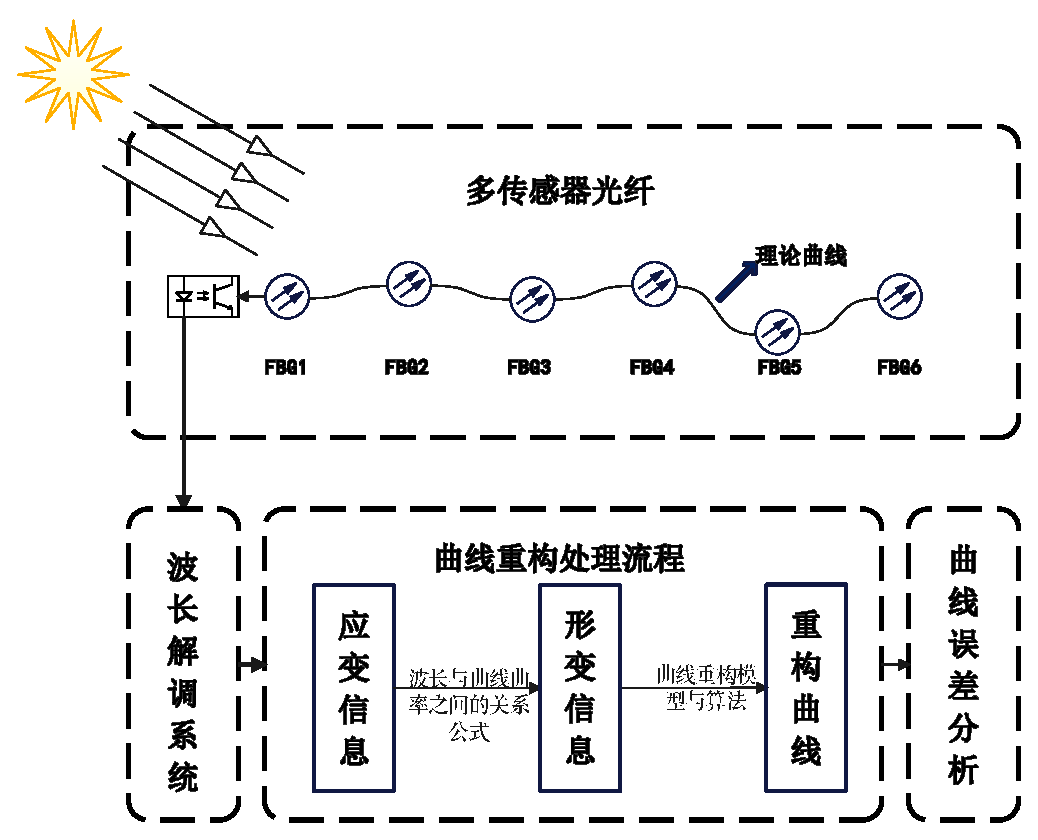
\includegraphics[width=.6\textwidth]{1.eps}
\caption{光纤传感器的平面曲线重建系统}
\end{figure}
\subsection{问题提出}
\begin{itemize}
\item 问题 1:根据题目给定的要求,光纤上布设的$6$个传感器间距为$0.6$米,已知两组的不同初始状态下受力前后的波长值和波长曲率关系公式,设计算法估算各个传感器的曲率。以初始点坐标为原点,初始方向为横轴,形变后初始点切线斜率为45度,建立模型求出给定横坐标处的曲线曲率。
\item 问题 2:基于问题一的曲率数据,建立数学模型,设计曲线重构算法并分析曲线特征。
\item 问题 3:根据题目给出的曲线方程$y=x^3+x(0 \leq x \leq 1)$,设计合适的距离进行等间距采样,获得采样点位置的曲率。基于采样点的曲率数据,结合问题二的模型算法,进行平面曲线重构,分析重构曲线和原始曲线的误差。
\end{itemize}


\section{问题分析}
根据题目给出光纤曲线重构问题,本文建立动力学模型来转化$(k,s)$坐标为$(x,y)$坐标,从而达到重构曲线的目的。
\subsection{问题一的分析}
根据题目要求,$6$个传感器间距为$0.6$米,并且两组的不同初始状态下受力前后的波长值和波长曲率关系公式已知。该问题是一个典型的插值与拟合问题。首先,我们通过波长曲率关系公式来估算测量点处的曲率;接着,通过三次样条插值法和多项式拟合法推得不同曲线长度下曲率值,进而根据形状重构原理,结合初始位置的坐标和切线方向,建立曲线在 xOy 坐标系下的微分方程,通过解微分方程得到横坐标的函数,通过数值积分方法得到横坐标的函数值,进而得到曲率信息。
\subsection{问题二的分析}
在问题一的基础上,分别得到$x$和$y$的对应坐标,然后对该曲线进行拟合得到重组曲线,再对重组曲线进行曲线特征分析。
\subsection{问题三的分析}
在已知函数曲线是$y=x^3+x$,先进行等弧长曲率采样,可以通过曲线积分得到弧长和横坐标的关系,再通过曲率公式得到曲率和横坐标关系,也就得到曲率和弧长的关系,采取等间距采样,得到离散的数据,再通过三次样条插值拟合得到曲率和弧长的函数,再通过建立的模型得到横纵坐标值,即可重构出曲线,再将重构曲线和原曲线对比分析误差。


\section{模型假设}
\begin{itemize}
\item 光纤在变形时为纯弯曲,忽略扭转对光纤长度的影响。
\item 光纤为一条曲线,忽略光纤的横截面积,仅考虑光纤的形状和长度。
\item 光纤仅存在于二维平面,不考虑光纤向z轴方向弯曲。
\item 光纤弯曲不会对传感器的测量产生影响。
\end{itemize}

\section{符号说明}
\begin{table}[H] % [htbp]是表格位置参数,可根据需要调整    
  \label{tab001} \centering     
  \begin{tabular}{c@{\hspace{6em}}c} % 定义表格列数及对齐方式,这里有两列,都居中对齐    
    \toprule[1.5pt] % 顶部粗线    
    符号   &   意义 \\ % 表格的表头    
    \midrule[1pt] % 中部细线    
    $s$   &   曲线弧长 \\ % 使用$...$来创建数学模式的下角标    
    $\theta_0$   &   曲线初始位置切线与水平轴的夹角 \\ % 同上    
    $k_(s)$   &   曲率-长度函数 \\ % 同上 
    $x_(t)$   &   重构曲线参数方程中$x$关于参数$t$的函数 \\ 
    $y_(t)$   &   重构曲线参数方程中$y$关于参数$t$的函数 \\  
    $\Delta L$   &   欧式距离 \\ 
    $k_i$   &   第$i$个各个测量点曲率 \\
    $S_i$   &   第$i$个取样点弧长 \\ 
    $X_i$   &   第$i$个各采样点横坐标 \\
    $K_i$   &   第$i$个各采样点曲率 \\  
    \bottomrule[1.5pt] % 底部粗线    
  \end{tabular}      
\end{table}

\section{动力学模型建立与求解}
\subsection{模型的原理与建立}
根据题目的要求,我们设想基于连续曲率函数实现曲线重构,建立以质点匀速运动轨迹为原理的动力学模型,模型具体如下:

\begin{figure}[!h]
\centering
\includegraphics[width=.6\textwidth]{0.pdf}
\caption{动力学模型原理示意图}
\end{figure}

设质点的运动关于时间$t$的参数方程为:
\begin{equation}
\left\{\begin{array}{l}
x=x(t) \\
y=y(t)
\end{array}\right.
\end{equation}

质点运动速度为$v$,在$x$轴和$y$轴的速度分量为$v_x$和$v_y$;质点运动加速度为$a$,在$x$轴和$y$轴的加速度分量为$a_x$和$a_y$;

$k=k(t)$ 表示 $\mathrm{t}$ 时刻的曲率;

$s=s(t)$ 表示 $\mathrm{t}$ 时刻的路程;

$\rho$ 表示质点在运动到$P$点对应的曲率半径;

\subsection{模型求解}
根据模型原理,由基础运动学公式推导得:

速度:
\begin{equation}
\begin{aligned}
& v_x=\dot{x} \\
& v_y=\dot{y} \\
& v=\sqrt{v_x^2+v_y^2}=\sqrt{\dot{x}^2+\dot{y}^2}
\end{aligned}
\end{equation}

加速度:
\begin{equation}
\begin{aligned}
& a_x=\ddot{x} \\
& a_y=\ddot{y} \\
& a=\sqrt{a_x{ }^2+a_y{ }^2}=\sqrt{\ddot{x}^2+\ddot{y}^2}
\end{aligned}
\end{equation}

由圆周运动规律可知,汽车在行驶到$P$点对应的向心加速度为:
\begin{equation}
a_n=\frac{v^2}{\rho}
\end{equation}

运动过的路程为:
\begin{equation}
s(t)=\int v d t
\end{equation}

\textbf{为简化计算,设质点的速率恒为$1$,则$s(t)=t$,$a=a_n$,推导得:} 
\begin{equation}
k=\frac{1}{\rho}=\frac{a}{v^2}=a
\end{equation}

带入$(3)$式可得:
\begin{equation}
k=\sqrt{\ddot{x}^2+\ddot{y}^2}
\end{equation}

接下来对$(2)$式的第三个公式两边对$t$求导可得:
\begin{equation}
\frac{\dot{x} \ddot{x}+\dot{y} \ddot{y}}{\sqrt{\dot{x}^2+\dot{y}^2}}=0
\end{equation}

由于 $v=\sqrt{\dot{x}^2+\dot{y}^2}=1$ ,故 $\ddot{x} \ddot{x}+\dot{y} \ddot{y}=0$ ,代入$(7)$式即可得:
\begin{equation}
\ddot{y}-k \sqrt{1-\dot{y}^2}=0
\end{equation}

令:
\begin{equation}
\left\{\begin{array}{l}
p=\dot{y} \\
\dot{p}-k \sqrt{1-p^2}=0
\end{array}\right.
\end{equation}

对于 $\dot{p}=k \sqrt{1-p^2}$ ,即 $\frac{d p}{d t}=k \sqrt{1-p^2}$ ,可得:
\begin{equation}
\frac{1}{\sqrt{1-p^2}} d p=k d t
\end{equation}

两边积分得到:
\begin{equation}
\arcsin p=\int k d t+C_1
\end{equation}

又由于$\dot{y}=p=\sin \left(\int k d t+C_1\right)$,两边积分得:
\begin{equation}
y=\int \sin \left(\int k d t+C_1\right) d t+C_2
\end{equation}

代入。。。式可得$\dot{x}=\cos \left(\int k d t+C_1\right)$,两边积分得:
\begin{equation}
x=\int \cos \left(\int k d t+C_1\right) d t+C_3
\end{equation}

\subsection{模型总结}
在已知曲率$k$关于$s$的表达式和曲线初始位置及参数后后,可由动力学模型得到$x$和$y$的坐标:
\begin{equation}
\left\{\begin{array}{l}
y=\int \sin \left(\int k d t+C_1\right) d t+C_2 \\
x=\int \cos \left(\int k d t+C_1\right) d t+C_3
\end{array}\right.
\end{equation}


\section{问题求解与模型评估}

\subsection{问题一 模型的建立与求解}
针对问题一,首先我们根据题目所给曲率公式,计算步长为$0.6$m的曲线长度对应的曲率值,然后建立分段连续曲率函数,通过三次样条插值法得到曲率-长度公式。根据上文建立的动力学模型,可以将所得的连续曲率函数转化为$xOy$坐标系下曲率的离散值。

\begin{figure}[!h]
\centering
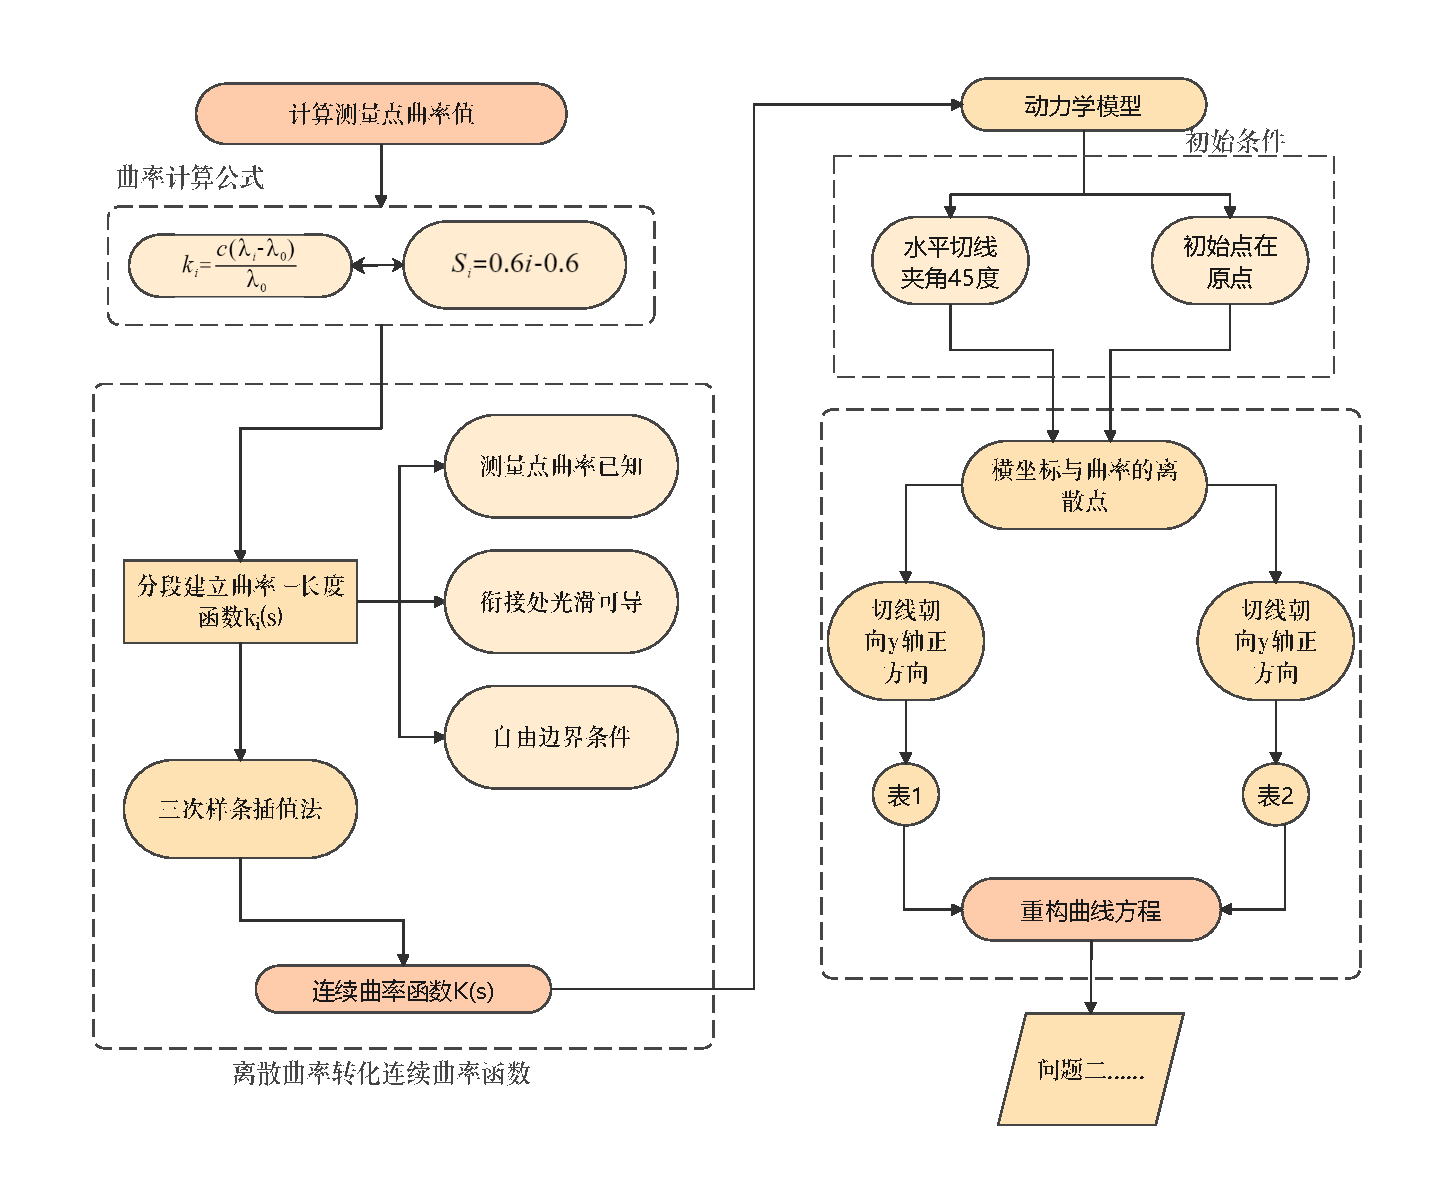
\includegraphics[width=.9\textwidth]{1mind.eps}
\caption{问题一思路图}
\end{figure}

\subsubsection{模型建立}
\textbf{测量点曲率:}  根据题目中给出的波长曲率公式和附件中的数据信息得到测量点FBG1~6的曲率,设向量$K_0$为测量点曲率集合,具体如下:
\begin{equation}
k_i=\frac{c\left(\lambda_i-\lambda_0\right)}{\lambda_0}, \quad i \in(1 , 6)\quad
\end{equation}
$k_i$代表第i个测量点的曲率,对应的曲线长度为$S_i$。
\begin{equation}
S_i=0.6 i-0.6\quad
\end{equation}

\textbf{建立曲率-长度函数:}  根据6个测量点的曲率和对应长度,建立曲率关于长度的函数,具体如下:,
\begin{equation}
k(s)=\left\{\begin{array}{lc}
k_1(s) & S_1 \leqslant s<S_2 \\
k_2(s) & S_2 \leqslant s<S_3 \\
k_3(s) & S_3 \leqslant s<S_4 \\
k_4(s) & S_4 \leqslant s<S_5 \\
k_5(s) & S_5 \leqslant s<S_6 
\end{array}\right.
\end{equation}


\subsubsection{利用三次样条插值法求解曲率函数}
三次样条插值法的基本原理就是采用分段插值把光纤分成5个区间,每个小区间的曲线是一个三次方程,在满足插值条件和曲线光滑的条件下可以得到足够的方程个数来求解未知参数。

\paragraph{建立三次函数}:

设$k_i(s)$为三次函数
\begin{equation}
k_i(s)=a_i \times\left(s-S_i\right)^3+b_i \times\left(s-S_i\right)^2+c_i \times\left(s-S_i\right)+d_i\quad
\end{equation}

由此建立系数向量:
\begin{equation}
\begin{aligned}
& P=\left[\begin{array}{llllll}
a_1 & b_1 & c_1 & d_1 & \ldots
\end{array}\right. \\
& \begin{array}{lllll}
a_2 & b_2 & c_2 & d_2 & \ldots
\end{array} \\
& \begin{array}{lllll}
a_3 & b_3 & c_3 & d_3 & \ldots
\end{array} \\
& \begin{array}{lllll}
a_4 & b_4 & c_4 & d_4 & \ldots
\end{array} \\
& \left.a_5 \quad b_5 \quad c_5 \quad d_5 \quad \cdots\right] \\
&
\end{aligned}\quad
\end{equation}

\textbf{约束条件:}

测量点曲率已知: 根据每个测量点的曲率值,可以确定每一段曲线的函数的初始值和结束值,则第$i$段曲线在$s_i$处对应的曲率为$k_i$,在$s_{i+1}$处对应的曲率为$k_{i+1}$:
\begin{equation}
\left\{\begin{array}{l}
k_i\left(S_i\right)=k_i \\
k_i\left(S_{i+1}\right)=k_{i+1}
\end{array}\right.
\end{equation}

曲线连续且光滑:根据题目所给条件,第$i$段曲线与第$i+1$段曲线的衔接处连续可导,即:
\begin{equation}
\left\{\begin{array}{l}
k_i^{\prime}\left(S_{i+1}\right)=k_{i+1}^{\prime}\left(S_{i+1}\right) \\
k_i^{\prime \prime}\left(S_{i+1}\right)=k_{i+1}^{\prime \prime}\left(S_{i+1}\right)
\end{array}\right.
\end{equation}

自然边界条件:端点二阶导数为0
\begin{equation}
\left\{\begin{array}{l}
k_1^{\prime \prime}\left(S_1\right)=0 \\
k_5^{\prime \prime}\left(S_6\right)=0
\end{array}\right.
\end{equation}

根据约束条件建立系数矩阵$M$和参数向量$V$,得到线性方程组:
\begin{equation}
M P=V\quad
\end{equation}

进而求出参数向量:
\begin{equation}
P=M^{-1} V\quad
\end{equation}

\paragraph{曲率函数}:
带入参数,得到曲率-长度的函数表达式:

测试1:
\begin{equation}
k_1(s) =
\begin{cases}
2.219 - 0.054s + 0.109s^2 - 0.046s^3 & 0 \leqslant s < 0.6 \\
2.217 + 0.028(s - 0.6) + 0.027(s - 0.6)^2 - 0.046(s - 0.6)^3 & 0.6 \leqslant s < 1.2 \\
2.233 + 0.010(s - 1.2) - 0.056(s - 1.2)^2 + 0.052(s - 1.2)^3 & 1.2 \leqslant s < 1.8 \\
2.230 - 0.001(s - 1.8) + 0.038(s - 1.8)^2 - 0.036(s - 1.8)^3 & 1.8 \leqslant s < 2.4 \\
2.236 + 0.006(s - 2.4) - 0.027(s - 2.4)^2 - 0.036(s - 2.4)^3 & 2.4 \leqslant s < 3.0
\end{cases}
\end{equation}

\begin{figure}[!h]
\centering
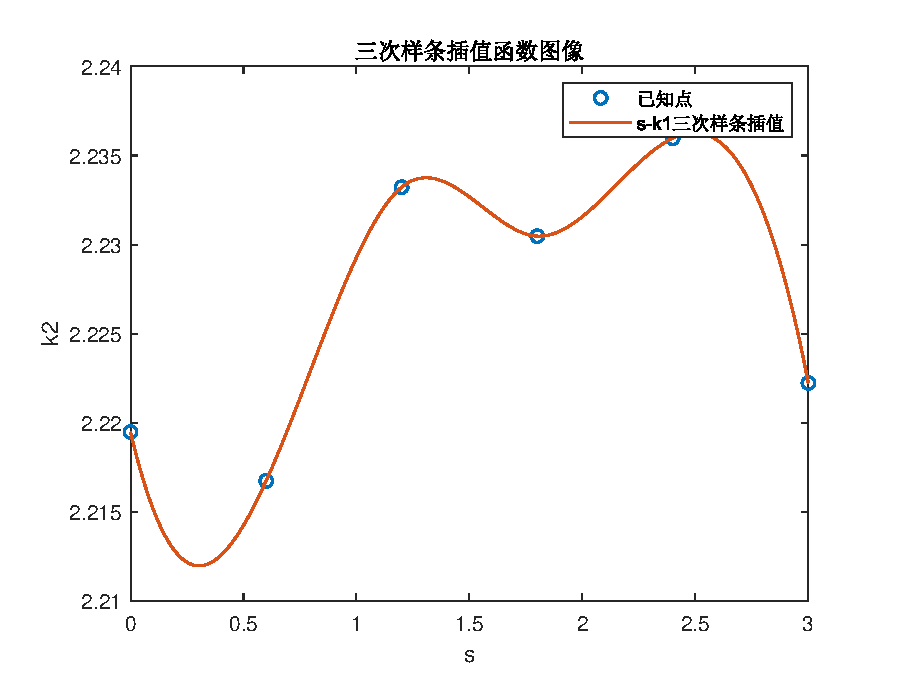
\includegraphics[width=.9\textwidth]{s-k1.eps}
\caption{测试1连续曲率函数$k_1(s)$}
\end{figure}

测试2:
\begin{equation}
k_2(s) =
\begin{cases}
2.986 - 0.005s -0.024s^2 + 0.015s^3 & 0 \leqslant s < 0.6 \\
2.978 - 0.017(s - 0.6) + 0.004(s - 0.6)^2 + 0.015(s - 0.6)^3 & 0.6 \leqslant s < 1.2 \\
2.973 + 0.004(s - 1.2) + 0.031(s - 1.2)^2 - 0.026(s - 1.2)^3 & 1.2 \leqslant s < 1.8 \\
2.981 + 0.014(s - 1.8) - 0.015(s - 1.8)^2 + 0.0001(s - 1.8)^3 & 1.8 \leqslant s < 2.4 \\
2.984 - 0.005(s - 2.4) - 0.015(s - 2.4)^2 + 0.0001(s - 2.4)^3 & 2.4 \leqslant s < 3.0
\end{cases}
\end{equation}

\begin{figure}[!h]
\centering
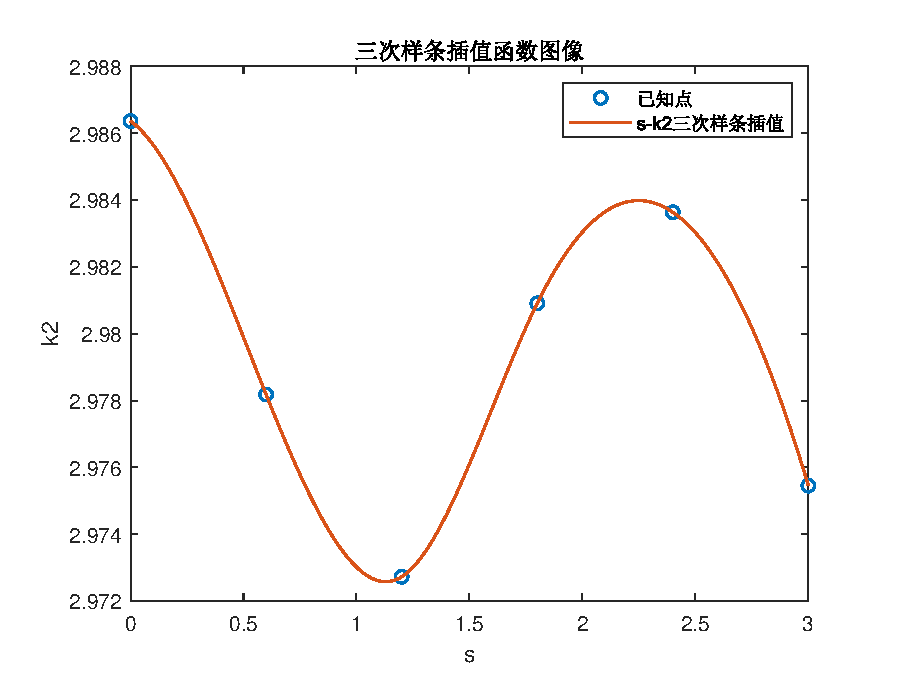
\includegraphics[width=.9\textwidth]{s-k2.eps}
\caption{测试2连续曲率函数$k_2(s)$}
\end{figure}

\subsubsection{动力学模型求解坐标对应曲率}
通过上文建立的动力学模型,可以得到$x$坐标与$k(s)$的关系式:
\begin{equation}
x=\int \cos \left(\int k d t+c_1\right)+c_3 .
\end{equation}

根据题目所给条件,已知曲线切线与水平方向的夹角为45度,曲线初始位置为坐标轴原点,即$\theta_0$为初始值$C_1$,$C_2$为$0$:
\begin{equation}
\begin{aligned}
& c_1=\theta_0= \pm \frac{\pi}{4} \\
& c_3=0
\end{aligned}
\end{equation}

由于$(28)$式没有解析解,故采用数值积分模型进行求解,常用的数值积分方法有:矩形法、梯形法、抛物线法等,在这里我们采用基于矩形法进行求解,原理如下:
\begin{figure}[!h]
\centering
\includegraphics[width=.9\textwidth]{jux.pdf}
\caption{矩形法积分原理示意图}
\end{figure}

对应公式为:
\begin{equation}
\int_0^{x_0} f(x) \mathrm{d} x=\sum_{i=0}^{x_0 / h} f(i h) h
\end{equation}


\paragraph{测试1}:


由于初始位置的的切线与水平方向的夹角$\theta_0$为45度,有可能朝向$y$轴的正方向和负方向,故列出以下两种情况。
\vspace{2cm}
\begin{figure}[!h]  
\centering  
\begin{minipage}{.5\textwidth}  
  \centering  
  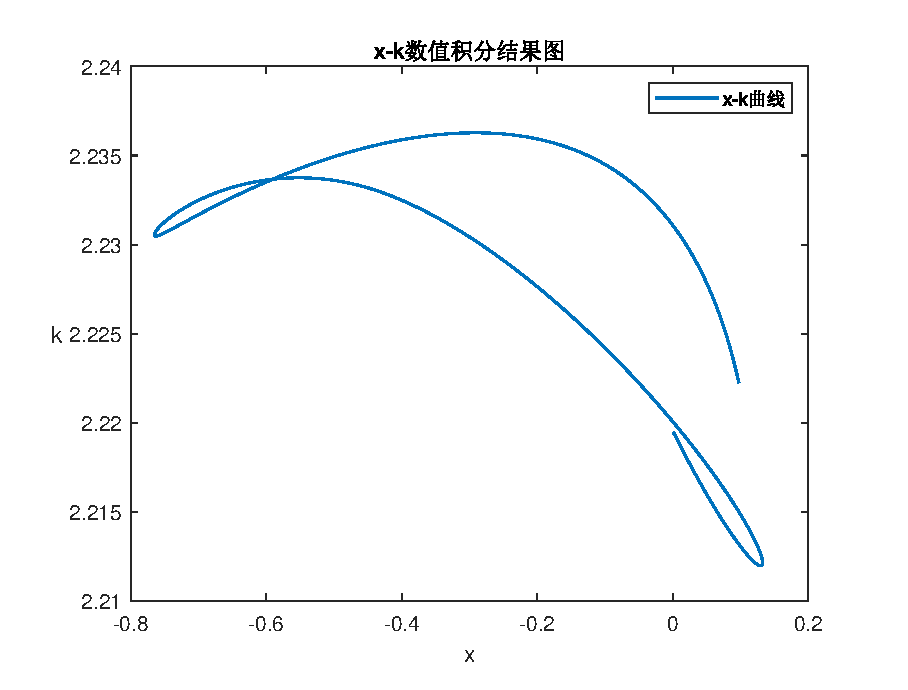
\includegraphics[width=.9\linewidth]{Q1x-k+45.eps}  
  \subcaption{$\theta_0=\frac{\pi}{4}$散点图}  
\end{minipage}%  
\begin{minipage}{.5\textwidth}  
  \centering  
  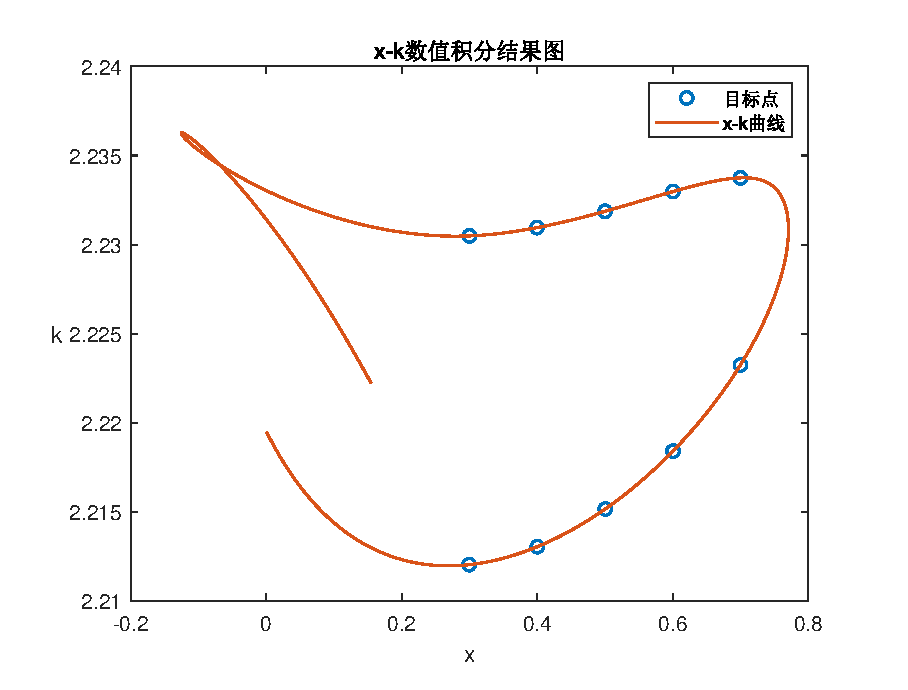
\includegraphics[width=.9\linewidth]{Q1x-k.eps}  
  \subcaption{$\theta_0=-\frac{\pi}{4}$散点图}  
\end{minipage}  
\caption{测试1散点图}  
\end{figure}  


当$\theta_0=\frac{\pi}{4}$时,所求横坐标超出曲线范围。

当$\theta_0=-\frac{\pi}{4}$时,从散点图可以看出曲线弯曲成椭圆状,且有重叠区域,故$x$坐标有多个对应的曲率值,下列表格按照距离曲线初始点的长度大小进行排序,如第二行则代表曲线第二次经过$x$坐标的曲率,具体可见附件$test1/_x-y.gif$和$test2/_x-y.gif$

\begin{table}[!h]  
\centering  
\begin{tabular}{|l|l|l|l|l|l|}  
\hline  
\text{横坐标 } $x$ \text{ (米) } & 0.3 & 0.4 & 0.5 & 0.6 & 0.7 \\  
\hline  
\text{曲率1 } $k$ & 2.2074 & 2.2100 & 2.2138 & 2.2186 & 2.2244 \\  
\hline  
\text{曲率2 } $k$ & 2.2299 & 2.2305 & 2.2314 & 2.2323 & 2.2330 \\  
\hline  
\end{tabular}  
\caption{不同横坐标下的曲率值}  
\label{tab:curvature_values}  
\end{table}  

值得注意的是,由于$\theta_0$只影响光纤初始位置的方向,而不改变光纤的形状,但由于无论$\theta_0=\frac{\pi}{4}$还是$\theta_0=-\frac{\pi}{4}$都无法得到完整的表格数据,所以在此另外列出曲线长度对应曲率的表格,图像参考图4:

\begin{table}[!h]  
\centering  
\begin{tabular}{|l|l|l|l|l|l|}  
\hline  
\text { 曲线长度 } s \text { (米) } & 0.3 & 0.4 & 0.5 & 0.6 & 0.7 \\
\hline   
\text { 测试 1 曲率 } k & 2.212 & 2.2126 & 2.2143 & 2.2167 & 2.2198 \\ 
\hline  
\end{tabular}  
\caption{不同曲线长度下的曲率值}  
\label{tab:curvature_values1}  
\end{table}  

\paragraph{测试2}:

\begin{figure}[!h]  
\centering  
\begin{minipage}{.5\textwidth}  
  \centering  
  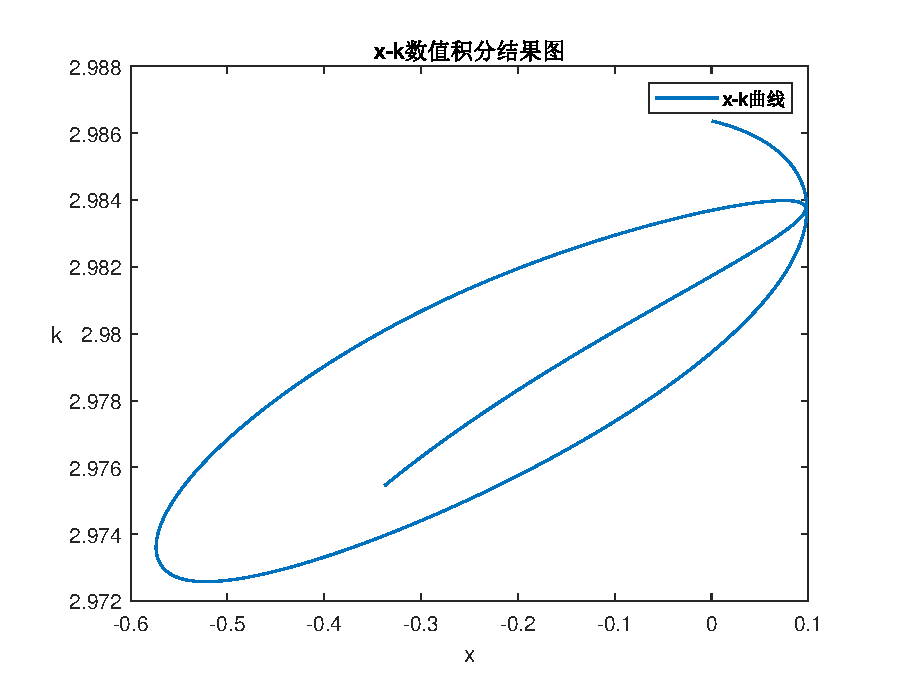
\includegraphics[width=.9\linewidth]{Q1x-k2+45.eps}  
  \subcaption{$\theta_0=\frac{\pi}{4}$散点图}  
\end{minipage}%  
\begin{minipage}{.5\textwidth}  
  \centering  
  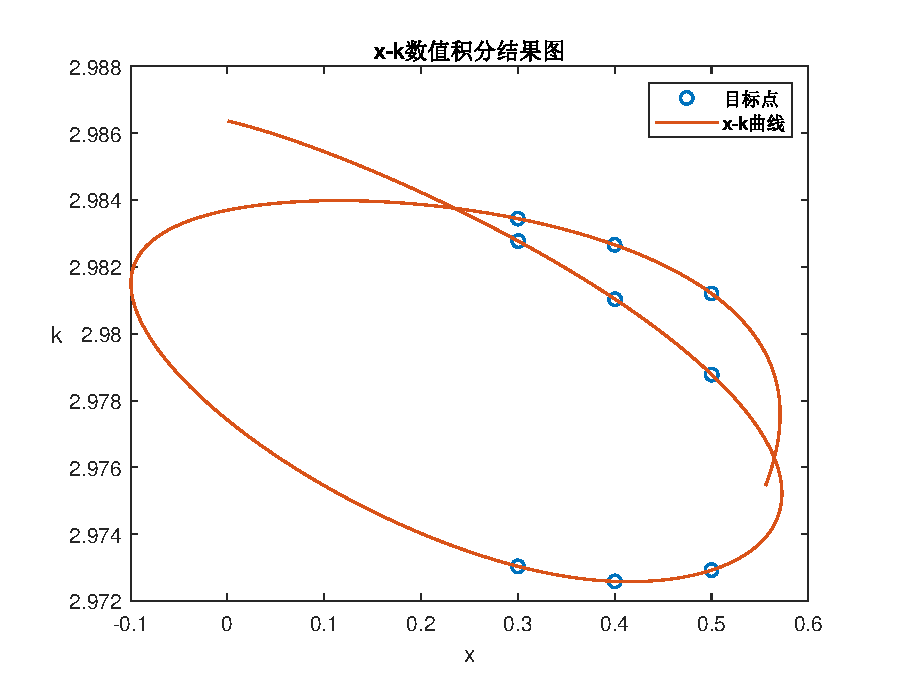
\includegraphics[width=.9\linewidth]{Q1x-k2.eps}  
  \subcaption{$\theta_0=-\frac{\pi}{4}$散点图}  
\end{minipage}  
\caption{测试2散点图}  
\end{figure}  


当$\theta_0=\frac{\pi}{4}$时,横坐标超出曲线范围。

当$\theta_0=-\frac{\pi}{4}$时,具体数据如下:

\begin{table}[!h]  
\centering  
\begin{tabular}{|l|l|l|l|l|l|}  
\hline  
\text{横坐标 } $x$ \text{ (米) } & 0.3 & 0.4 & 0.5 & 0.6 & 0.7 \\  
\hline  
\text{曲率1 } $k$ & 2.9841 & 2.9817 & 2.9786 & \text{ 无 } & \text{ 无 } \\  
\hline  
\text{曲率2 } $k$ & 2.9728 & 2.9721 & 2.9721 & \text{ 无 } & \text{ 无 } \\  
\hline  
\text{曲率3 } $k$ & 2.9833 & 2.9821 & 2.9801 & \text{ 无 } & \text{ 无 } \\  
\hline  
\end{tabular}  
\caption{测试2不同横坐标下的曲率值}  
\label{tab:curvature}  
\end{table}  

\vspace{7cm}

由于无法得到完整的表格数据,故在此另外列出曲线长度对应曲率的表格,即曲线长度对应曲率,图像参考图5:
\begin{table}[!h]  
\centering  
\begin{tabular}{|l|l|l|l|l|l|}  
\hline  
\text { 曲线长度 } s \text { (米) } & 0.3 & 0.4 & 0.5 & 0.6 & 0.7 \\
\hline  
\text { 测试 1 曲率 } k & 2.9832 & 2.9816 & 2.9799 & 2.9782 & 2.9765 \\
\hline  
\end{tabular}  
\caption{测试2不同横坐标下的曲率值}  
\label{tab:curvature}  
\end{table}

\subsection{问题二 模型的建立与求解}

\subsubsection{模型建立}
根据动力学模型,建立光纤重构曲线参数方程:
\begin{equation}
\left\{\begin{array}{l}
x=x(t) \\
y=y(t)
\end{array}\right.
\end{equation}


\subsubsection{利用动力学模型法求离散坐标值}
根据问题一中的三次样条插值法,将离散曲率函数转化为连续曲率函数$k(s)$,再通过$(14)$式可求解得到离散的坐标值,由于$(14)$式的积分函数没有解析解,在此我们利用矩形法进行数值运算,原理如图所示:


在MATLAB中设置矩形法步长为$0.001$,$t$的范围0$~$3,取3000个样本,绘图如下;

$xOy$坐标系:

测试1:
\begin{figure}[!h]  
\centering  
\begin{minipage}{.5\textwidth}  
  \centering  
  \includegraphics[width=.9\linewidth]{k1+45.eps}  
  \subcaption{$\theta_0=-\frac{\pi}{4}$散点图1}  
\end{minipage}%  
\begin{minipage}{.5\textwidth}  
  \centering  
  \includegraphics[width=.9\linewidth]{k1_san.eps}  
  \subcaption{$\theta_0=-\frac{\pi}{4}$散点图2}  
\end{minipage}  
\caption{测试1散点图}  
\end{figure} 

测试2:
\begin{figure}[!h]  
\centering  
\begin{minipage}{.5\textwidth}  
  \centering  
  \includegraphics[width=.9\linewidth]{k2+45.eps}  
  \subcaption{$\theta_0=-\frac{\pi}{4}$散点图1}  
\end{minipage}%  
\begin{minipage}{.5\textwidth}  
  \centering  
  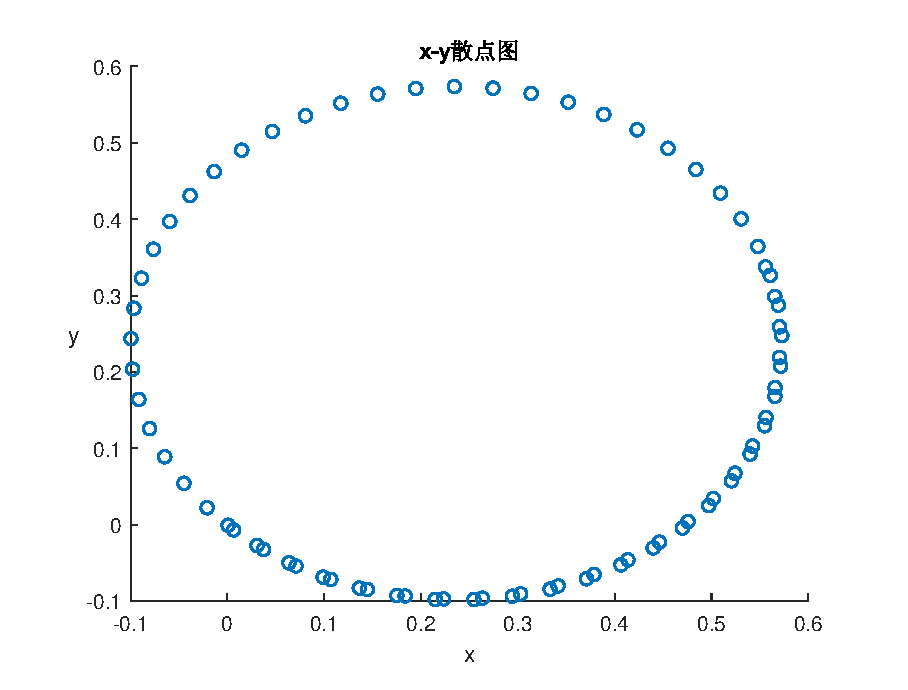
\includegraphics[width=.9\linewidth]{k2_san.eps}  
  \subcaption{$\theta_0=-\frac{\pi}{4}$散点图2}  
\end{minipage}  
\caption{测试2散点图}  
\end{figure}  

极坐标系:
\begin{figure}[!h]
\centering
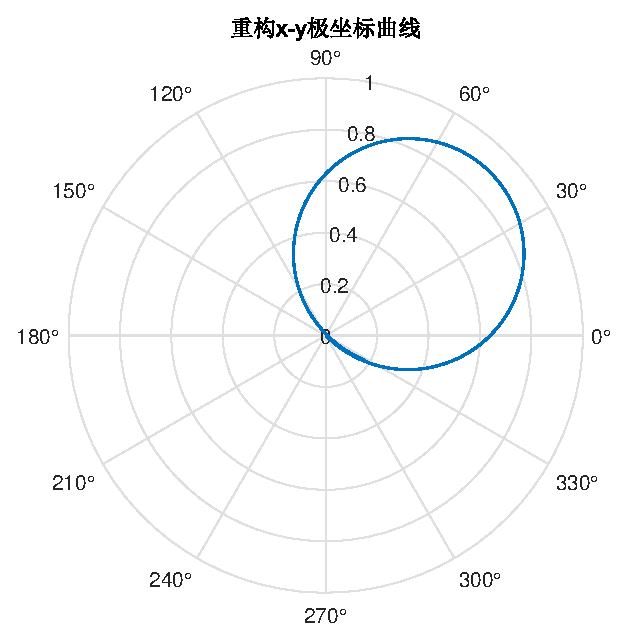
\includegraphics[width=.6\textwidth]{1极坐标.eps}
\caption{测试1极坐标系示意图}
\end{figure}

\begin{figure}[!h]
\centering
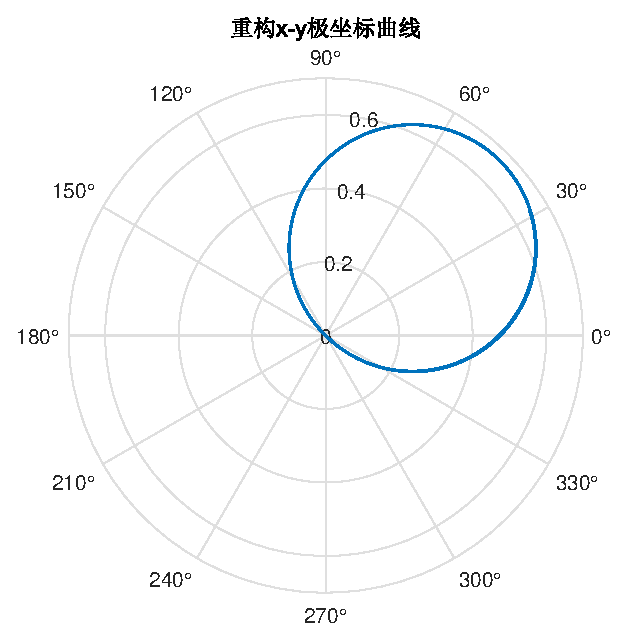
\includegraphics[width=.6\textwidth]{2极坐标.eps}
\caption{测试2极坐标系示意图}
\end{figure}

\vspace{8cm}

\subsubsection{利用多项式拟合法求曲率方程}
基于以上离散坐标值通过多项式拟合函数polyfit进行7阶多项式拟合,得到对应的$x(t)$和$y(t)$,结果如下:

\textbf{测试1}
\begin{equation}
\left\{\begin{array}{l}
x(t)=0.015 t^7-0.184 x^6+0.797 x^5-1.271 t^4+0.166 t^3+0.487 t^2+0.756 t-0.001 \\
y(t)=-0.01 t^7+0.062 t^6+0.026 t^5-0.749 t^4+1.029 t^3+0.565 t^2-0.664 t-0.003
\end{array}\right.
\end{equation}

具体如下:
\begin{figure}[!h]  
\centering  
\begin{minipage}{.5\textwidth}  
  \centering  
  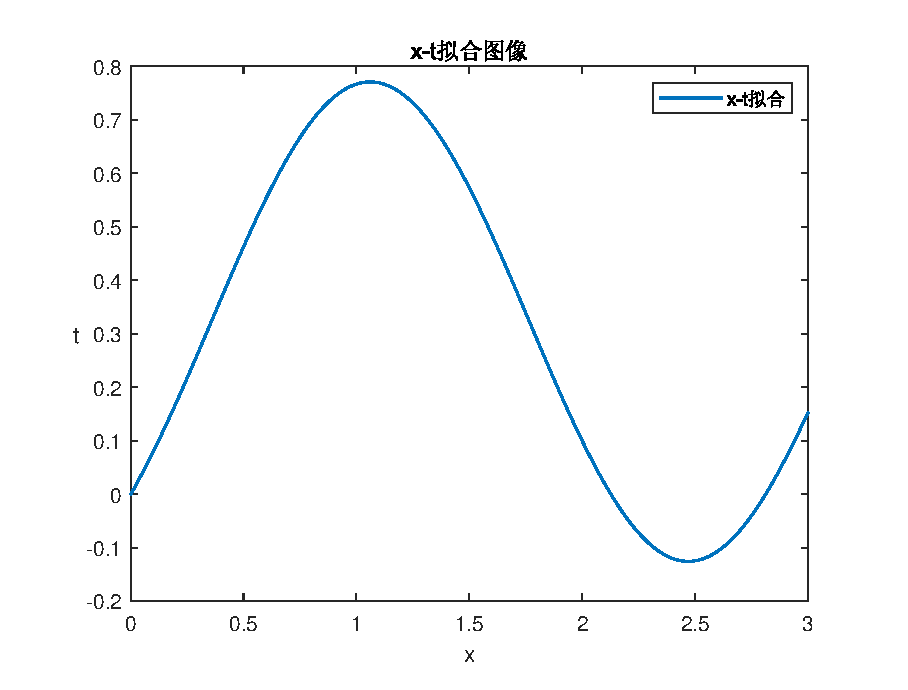
\includegraphics[width=.9\linewidth]{1x-t拟合.eps}  
  \subcaption{$x(t)$拟合曲线}  
\end{minipage}%  
\begin{minipage}{.5\textwidth}  
  \centering  
  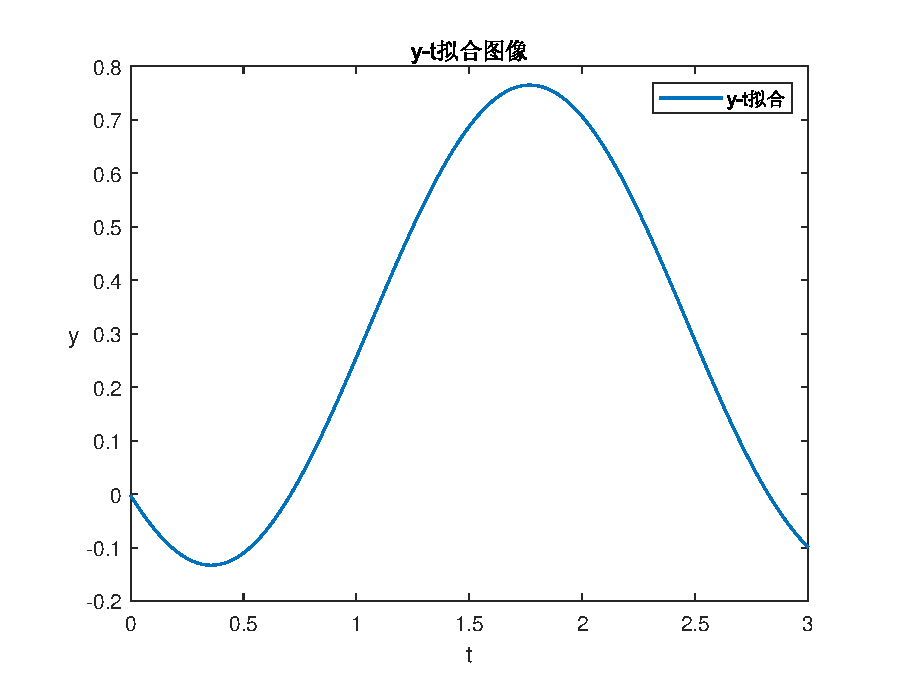
\includegraphics[width=.9\linewidth]{1y-t拟合.eps}  
  \subcaption{$y(t)$拟合曲线}  
\end{minipage}  
\caption{测试1重构曲线}  
\end{figure}  

\textbf{测试2}
\begin{equation}
\left\{\begin{array}{l}
x(t)=0.015 t^7-0.184 x^6+0.797 x^5-1.271 t^4+0.166 t^3+0.487 t^2+0.756 t-0.001 \\
y(t)=-0.01 t^7+0.062 t^6+0.026 t^5-0.749 t^4+1.029 t^3+0.565 t^2-0.664 t-0.003
\end{array}\right.
\end{equation}

具体如下:
\begin{figure}[!h]  
\centering  
\begin{minipage}{.5\textwidth}  
  \centering  
  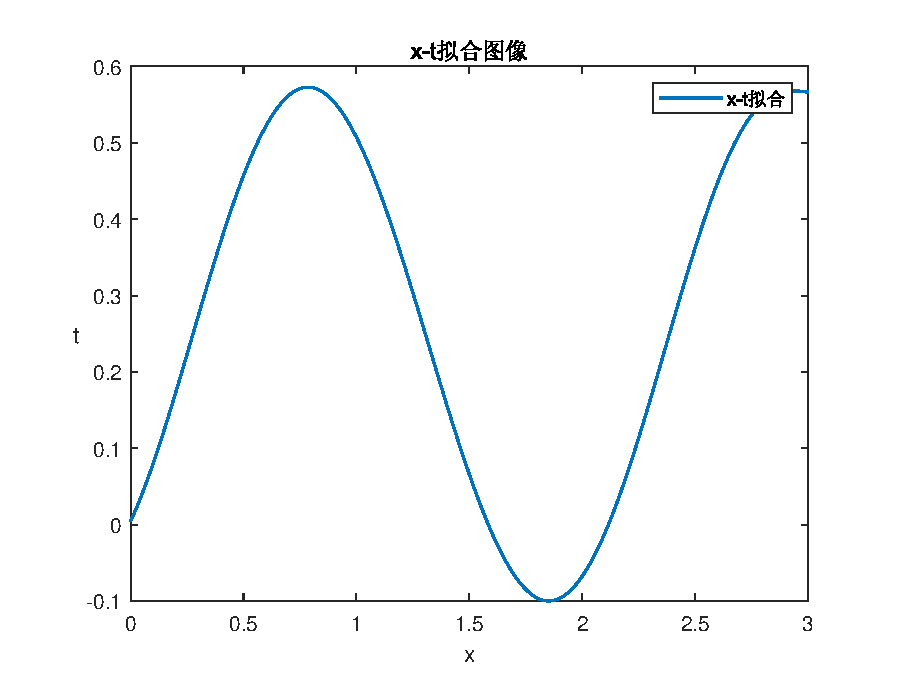
\includegraphics[width=.9\linewidth]{2x-t拟合.eps}  
  \subcaption{$x(t)$拟合曲线}  
\end{minipage}%  
\begin{minipage}{.5\textwidth}  
  \centering  
  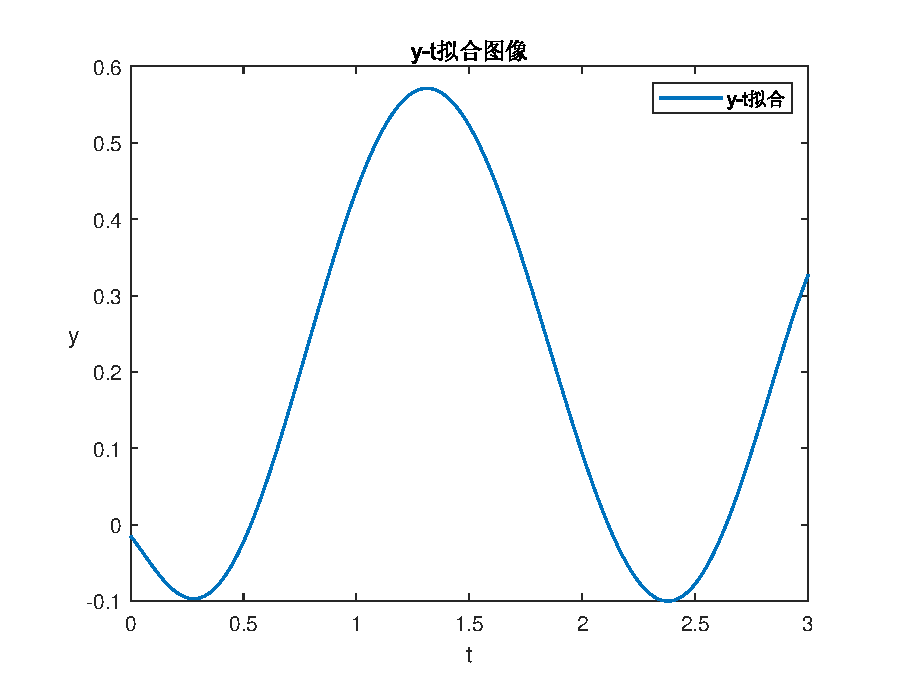
\includegraphics[width=.9\linewidth]{2y-t拟合.eps}  
  \subcaption{$y(t)$拟合曲线}  
\end{minipage}  
\caption{测试2重构曲线}  
\end{figure} 


\subsubsection{曲线特征分析}
\begin{itemize}
\item 形状与方向:重构曲线的整体形状为椭圆形,在部分范围内有交叠情况。
\item 光滑性:曲线的重构结果光滑连续,不存在突变或不自然的转折点,曲率变化合理。
\item 物理意义:光纤具有质地轻、体积小、弯曲性能好等特性,便于获得结构的应变信息,重建结构的形状,该重构曲线也较符合光纤的实际应用情景,如对结肠部位进行形状重建等。
\end{itemize}

\subsection{问题三 模型的建立与求解}
针对问题三,我们需要在解决问题一和问题二的基础上,对平面曲线方程$y=x^3+x(0 \leq x \leq 1)$根据弧长进行等间距采样并重构曲线方程,利用Runge-Kutta法计算曲线弧长s,得到弧长s与横坐标x之间的关系,从而得到步长为$0.22$m时的曲线曲率。

得到离散曲率信息后,可以利用问题一的三次样条插值法求得连续曲率函数。随后运用构建的动力学模型得到重构曲线的大量离散点,将离散点通过多项式拟合得到重构曲线。

最后对比重构曲线方程和原始曲线方程,通过计算欧式距离误差进行误差分析。

\subsubsection{等间距弧长采样}
根据曲线的弧长积分公式$d s=\sqrt{1+\left(y^{\prime}\right)^2} d x$ 得到弧长s与横坐标x之间的关系,即:
\begin{equation}
d s=\sqrt{1+\left(3 x^2+1\right)} d x
\end{equation}

由于该微分方程没有解析解,故采用Runge-Kutta法求s对x的离散数值解,Runge-Kutta法的主要思路是利用区间内特定点的一阶导数值的线性组合来近似某点的高阶导数值,进而迭代求解微分方程或方程组的数值解。此方法通过将微分方程离散化,建立差分方程,并通过已知的初始条件逐步计算出解在一系列点上的近似值。

绘制对应离散数值解如下图所示:
\begin{figure}[!h]
\centering
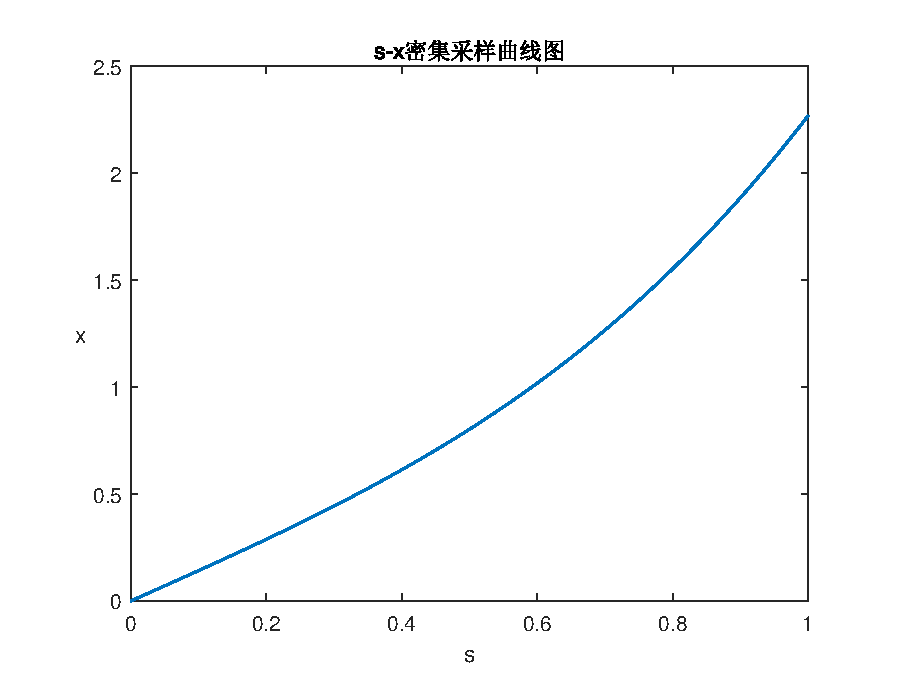
\includegraphics[width=.5\textwidth]{Q3.eps}
\caption{弧长s和横坐标x的离散数值解}
\end{figure}

 % 在这里插入1厘米的垂直空白  
\vspace{6cm}

基于s与x的离散数值解,取弧长采样间隔为$0.22$,得到采样点长度向量$S_1$根据离散数值解得$S_1$对应的横坐标向量$X_1$,根据曲率公式$k=\frac{\left|y^{\prime \prime}\right|}{\left(1+y^{\prime 2}\right)^{\frac{3}{2}}}$和原函数公式$y=x^3+x(0 \leq x \leq 1)$,得到S1对应的曲率为下表:
\begin{table}[!h]  
\centering  
\begin{tabular}{|c|c|c|c|c|c|c|c|c|c|c|}  
\hline  
\text { 曲线长度 } s \text { (米) } & 0.220 & 0.440 & 0.660 & 0.880 & 1.100 & 1.320 & 1.540 & 1.760 & 1.980 & 2.200 \\ \hline  
\text { 曲率 } k & 0.293 & 0.425 & 0.411 & 0.340 & 0.268 & 0.209 & 0.166 & 0.133 & 0.109 & 0.091 \\ \hline  
\end{tabular}  
\caption{等间隔采样点下的曲率值}  
\label{tab:curvature}  
\end{table}

\subsubsection{利用插值法求曲率函数}
已知采样点长度及曲率大小,通过三次样条插值法得到连续采样函数,求解原理同问题一:

\begin{equation}  
S(x) =  
\begin{cases}  
0.000 + 1.686x - 1.576x^2 - 0.133x^3 & 0 \leqslant x < 0.22 \\  
0.293 + 0.973(x - 0.22) - 1.664(x - 0.22)^2 - 0.133(x - 0.22)^3 & 0.22 \leqslant x < 0.44 \\  
0.425 + 0.222(x - 0.44) - 1.751(x - 0.44)^2 + 1.988(x - 0.44)^3 & 0.44 \leqslant x < 0.66 \\  
0.411 - 0.260(x - 0.66) - 0.440(x - 0.66)^2 + 0.733(x - 0.66)^3 & 0.66 \leqslant x < 0.88 \\  
0.34 - 0.347(x - 0.88) + 0.044(x - 0.88)^2 + 0.191(x - 0.88)^3 & 0.880 \leqslant x < 1.1 \\  
0.268 - 0.301(x - 1.1) + 0.169(x - 1.1)^2 - 0.026(x - 1.1)^3 & 1.1 \leqslant x < 1.32 \\  
0.209 - 0.23(x - 1.32) + 0.152(x - 1.32)^2 - 0.055(x - 1.32)^3 & 1.32 \leqslant x < 1.54\\  
0.166 - 0.171(x - 1.54) + 0.116(x - 1.54)^2 - 0.050(x - 1.54)^3 & 1.54 \leqslant x < 1.76 \\  
0.133 - 0.127(x - 1.76) + 0.083(x - 1.76)^2 - 0.034(x - 1.76)^3 & 1.76 \leqslant x < 1.98 \\  
0.109 - 0.095(x - 1.98) + 0.061(x - 1.98)^2 - 0.034(x - 1.98)^3 & 1.98 \leqslant x < 2.2  
\end{cases}  
\end{equation}
\subsubsection{利用动力学模型曲线重构}
根据连续采样函数和动力学模型,可得到一系列离散样本的曲率值,通过对离散点进行多项式拟合得到重构曲线方程。

多项式拟合结果:
\begin{equation}
y=1.012916x^3-0.008591x^2+1.002926x-0.000847
\end{equation}

拟合绘图如下:
\begin{figure}[!h]
\centering
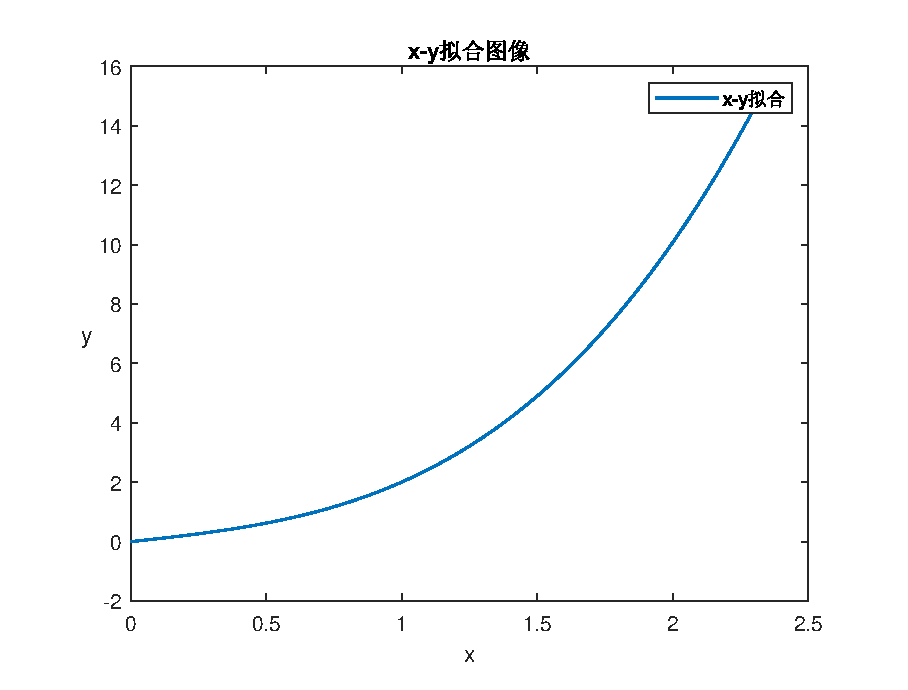
\includegraphics[width=.6\textwidth]{x-y拟合.eps}
\caption{拟合示意图}
\end{figure}


\subsubsection{误差分析}
重构曲线与原始曲线对比图如下:
\begin{figure}[!h]
\centering
\includegraphics[width=.8\textwidth]{Q3_11.pdf}
\caption{重构曲线与原始曲线图}
\end{figure}


由于该题的实际意义是光纤实体,我们将光纤的形状用函数$y=x^3+x$表达,故在分析误差时,我们不采用$
\left(y-y^{\prime}\right)-x $的误差图线,而采用更具实际意义的$\Delta L-\mathrm{s}$误差分析,$\Delta L$表示原函数于拟合函数在同一弧长处的空间距离,即:
\begin{equation}
\Delta L=\sqrt{(x-\hat{x})^2+(y-\hat{y})^2}
\end{equation}

$\Delta L-\mathrm{s}$误差分析具体结果如下:
\begin{figure}[!h]
\centering
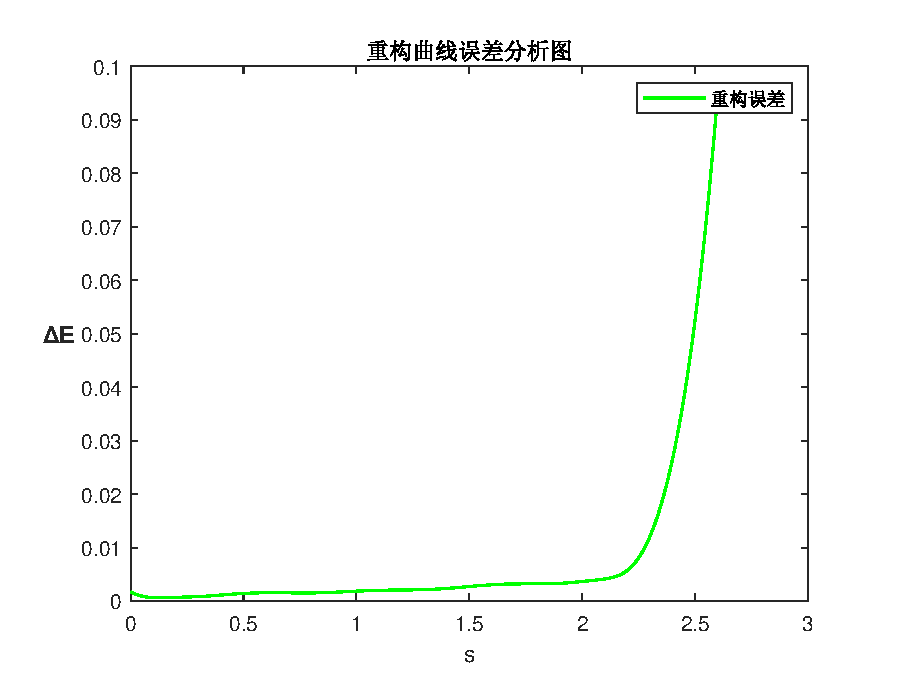
\includegraphics[width=.6\textwidth]{Q3误差.eps}
\caption{欧式距离误差分析图}
\end{figure}

\vspace{4cm}

由图像可以看到当$s$较小时,误差较小,当$s$较大时,误差较大,这是在求解重构曲线时,是使用四阶龙格库塔法求微分方程数值解,而该方法会在$s$增大时累计误差。但整体误差在$0.1$以下,在可接受范围内。$\Delta L$的平均值为$0.0072$,方差为$2.4086 \times 10^{-4}$。故可以得出,整体的重构曲线与原函数拟合较为准确。

\textbf{误差产生原因分析}:
\begin{itemize}
\item 三次样条插值虽然在少样本情况下有更好的效果,但是其所得的曲线仍和实际情况有误差,且这个误差不可避免。
\item 多项式拟合大样本数据时可能会存在区间短点处的误差较大,且有可能会陷入曲线震荡的困境。
\item 矩形法数值积分的精度较低,故可能会产生较大的误差。
\item 龙格库塔法求解微分方程数值解时会有内在误差。
\end{itemize}


\section{模型的评价与推广}
\subsection{模型的优点}
\textbf{问题一模型优点}:

模型一采用三次样条插值模型对题目中给出的$6$个数据进行插值,相比较一般的拟合方法,三次样条插值对于少量离散数据的拟合更为准确,而使用七次多项式拟合的方式对所求得的大量$(x,s)$的数据进行拟合,相较于插值方法,多项式拟合在处理大量数据时更有优势。在将$(k,s)$数据转变成$(x,s)$数据时,采用定积分的方法进行数值积分。该方法具有适用性广,且较为简便的特点。

\textbf{问题二模型优点}:

与问题一相同,用七次多项式拟合$(x,t)$,$(y,t)$图线,即得到重构曲线的参数方程,使用直角坐标系,极坐标系,参数方程的三种方式进行曲线的重构,能够从不同角度对重构曲线进行特征提取,也可以得到更多的曲线信息。

\textbf{问题三模型优点}:

在抽取采样点时,由于无法得到函数$y=x^3+x$的弧长公式的解析解,故我们采用四阶龙格库塔模型求解数值解,该模型在求解数值解时精度较高,更贴近真实值。然后同样使用多项式拟合的方法得到$(k,s)$曲线,故可以精准取到等曲线间距时的曲率信息,再通过问题一和问题二的模型进行重构。与问题一二不同的是,由于该函数是单调的,故在得到$(x,t)$,$(y,t)$数据时我们采用了精度更高的四阶龙格库塔法,得到的结果也更为精确。在误差分析时,本文采用更具有实际意义的$\Delta L-\mathrm{s}$误差图,更能反应重组后的光纤曲线和真实光纤曲线的实际误差。

\subsection{模型的缺点}
\begin{itemize}
\item 限制性:模型可能只适用于平面二维曲线重构,且要求物体在变形时为纯弯曲。
\item 精确性:动力学模型重构的曲线方程的结果与实际结果存在偏差。
\end{itemize}

\subsection{模型的改进}
在进行数值积分时候,可以采用梯形法或者左矩形和右矩形法的中值,通过比较不同方法采取更为精确的积分结果。

在进行拟合和插值时,也可以通过采取不同的方法来进行比较,采取更精确的结果。
\subsection{模型的推广}
本文使用的动力学模型不仅在本题中可以得到相对精确的结果,更是给出了数学中函数图线信息$(s,k)$转化为$(x,y)$坐标的模型,这个模型可以解决更多的物理实际问题,比如道路平坦度曲线重构,汽车行驶轨迹重构等等。具有很强的普适性。

\vspace{5cm}

\begin{thebibliography}{1.2}%宽度9
\setlength{\itemsep}{-2mm}
 \bibitem{bib:one} 
 邵云. 力学中二维曲线曲率半径的表达式研究[J]. 高师理科学刊, 2021,41(05):39-43.
 \bibitem{bib:two}
 尚秋峰.刘峰.FBG形状传感器的曲率和弯曲方向误差修正模型[J]. 光学学报, 2023.
 \bibitem{bib:two}
 张晓晶,武湛君,张博明,等.光纤布拉格光栅温度和应变交叉灵敏度的实验研究[J]. 光电子·激光, 2005.
  \bibitem{bib:two}
 张俊,陈光辉,倪国新,等. FBG传感技术在飞机机翼动态形变监测中的应用[J].仪器仪表学报, 2023.
\end{thebibliography}

\newpage
%附录
\appendix

\section{程序代码}
%设置不同语言即可。
\begin{lstlisting}[language=Matlab] 
%波长转换为曲率
clc,clear
lambda1=[1529 1529 1529 1529 1529 1529];%初始状态1波长
lambda01=[1529.808 1529.807 1529.813 1529.812 1529.814 1529.809];%测试1

lambda2=[1540 1540 1540 1540 1540 1540];%初始状态2
lambda02=[1541.095 1541.092 1541.09 1541.093 1541.094 1541.091];%测试2
k1=4200*(lambda01-lambda1)./lambda1;
k2=4200*(lambda02-lambda2)./lambda2;
d1=[0.6 0.6 0.6 0.6 0.6 0.6];
d2=[0 0.6 1.2 1.8 2.4 3];

%插值得s-k图像
pp=spline(d2,k1);

% 使用pp结构体生成插值函数的分段多项式表达式(可选)
for i = 1:length(d2)-1
    fprintf('For x in [%f, %f]:\nS(x) = %f + %f*(x-%f) + %f*(x-%f)^2 + %f*(x-%f)^3\n\n', ...
            pp.breaks(i), pp.breaks(i+1), pp.coefs(i,4), pp.coefs(i,3), pp.breaks(i), ...
            pp.coefs(i,2), pp.breaks(i), pp.coefs(i,1), pp.breaks(i));

end

% 绘制插值函数图像
xx = linspace(min(d2), max(d2), 1000); % 生成密集的插值点横坐标
yy = ppval(pp, xx); % 利用pp结构体计算对应的插值点纵坐标

h=plot(d2, k1, 'o', xx, yy, '-', 'linewidth', 1.1); % 绘制原始数据点('o')及插值曲线
xlabel('x');
ylabel('y');
title('三次样条插值函数图像');

legend( h, '已知点', 's-k1三次样条插值', 'Location', 'NorthEast', 'Interpreter', 'none' );
% 为坐标区加标签
xlabel( 's', 'Interpreter', 'none' );
ylabel( 'k1', 'Interpreter', 'none' );
 \end{lstlisting}

\begin{lstlisting}[language=Matlab] 
%s-k1得x-y,数值积分
close all
h=0.001;%步长
t=0:h:3;
%插值得到的s-k1函数
k= ((2.219490 -0.053768*t + 0.109621*t.^2  -0.046064*t.^3).*(t>=0 & t<=0.6)+...
   (2.216743 + 0.028028*(t-0.6) + 0.026706*(t-0.6).^2 -0.046064*(t-0.6).^3).*(t>0.6 & t<=1.2)+...
   ( 2.233224 + 0.010326*(t-1.2) -0.056210*(t-1.2).^2 + 0.052281*(t-1.2).^3).*(t>1.2 & t<=1.8)+...
   (2.230477 + -0.000661*(t-1.8) + 0.037897*(t-1.8).^2 -0.035890*(t-1.8).^3).*(t>1.8 & t<=2.4)+...
   ( 2.235971 + 0.006053*(t-2.4) -0.026706*(t-2.4).^2  -0.035890*(t-2.4).^3).*(t>2.4 & t<=3));
%通过数值积分求解x、y
dtheta=zeros(length(t),1);
for i=1:length(t)-1
    if i==1
        dtheta(i)=h*k(i);
    end
    dtheta(i+1)=dtheta(i)+h*k(i);
end
theta=dtheta-pi./4;
y_1=sin(theta);
y=zeros(length(t),1);
for i=1:length(t)-1
    if i==1
        y(i)=h*y_1(i);
    end
    y(i+1)=y(i)+h*y_1(i);
end

x_1=cos(theta);
x=zeros(length(t),1);
for i=1:length(t)-1
    if i==1
        x(i)=h*x_1(i);
    end
    x(i+1)=x(i)+h*x_1(i);
end
figure
h=plot(x,k,'-', 'linewidth', 1.1)
xlabel('x');
ylabel('k','Rotation',0);
title('x-k数值积分结果图');
legend( h,  'x-k曲线', 'Location', 'NorthEast', 'Interpreter', 'none' );

figure
x1=[0.299532076
0.400096177
0.500336742
0.600358371
0.699807371
0.299975616
0.39958398
0.499984923
0.600217444
0.699847271

];
k1=[2.212044037
2.213052293
2.215167342
2.218418833
2.223247381
2.230490013
2.230952812
2.231870715
2.232977507
2.233746417
];
h=plot(x1,k1,'o',x,k,'-', 'linewidth', 1.1);
xlabel('x');
ylabel('k','Rotation',0);
title('x-k数值积分结果图');
legend( h, '目标点', 'x-k曲线', 'Location', 'NorthEast', 'Interpreter', 'none' );

figure;
%拟合x-t
P1=polyfit(t,x,7);
yy=polyval(P1,t);
fprintf('%f *x.^7+%f *t.^6+%f *t.^5+%f *t.^4+%f *t.^3+%f *t.^2+%f *t+ %f', ...
    P1(1),P1(2),P1(3),P1(4),P1(5),P1(6),P1(7),P1(8));
h1=plot(t,yy,'-', 'linewidth', 1.1);
xlabel('x');
ylabel('t','rotation',0);
title('x-t拟合图像');
legend( h1, 'x-t拟合', 'Location', 'NorthEast', 'Interpreter', 'none' );
%误差分析
figure;
dy=yy'-x;
h2=plot(t,dy,'-', 'linewidth', 1.1,'color','g')
xlabel('t');
ylabel('dx','rotation',0);
title('拟合误差图像');
legend( h2, 'x-t拟合误差', 'Location', 'NorthEast', 'Interpreter', 'none' );

%拟合y-t
figure;
P2=polyfit(t,y,7);
yy=polyval(P2,t);
fprintf('%f *x.^7+%f *t.^6+%f *t.^5+%f *t.^4+%f *t.^3+%f *t.^2+%f *t+ %f', ...
    P2(1),P2(2),P2(3),P2(4),P2(5),P2(6),P2(7),P2(8));
h3=plot(t,yy, 'linewidth', 1.1);
xlabel('t');
ylabel('y','rotation',0);
title('y-t拟合图像');
legend( h3, 'y-t拟合', 'Location', 'NorthEast', 'Interpreter', 'none' );

%误差分析
figure;
dy=yy'-y;
h4=plot(t,dy,'linewidth', 1.1,'color','g')
xlabel('t');
ylabel('dy','rotation',0);
title('拟合误差图像');
legend( h4, 'y-t拟合误差', 'Location', 'NorthEast', 'Interpreter', 'none' );

%重构x-y曲线(笛卡尔坐标系)
figure;
h5=plot(x,y,'linewidth', 1.1);
xlabel('x');
ylabel('y','rotation',0);
title('重构x-y曲线');
legend( h5, 'x-y曲线', 'Location', 'NorthEast', 'Interpreter', 'none' );

%极坐标系下展示
figure
p=(x.^2+y.^2).^(1./2);
h6=polarplot(atan2(y,x),p,'linewidth', 1.1)
title('重构x-y极坐标曲线');

figure
x11=x(1:40:end);
y11=y(1:40:end);
h7=scatter(x11,y11,'linewidth', 1)
xlabel('x');
ylabel('y','rotation',0);
title('x-y散点图');
legend( h7, '重构曲线散点', 'Location', 'NorthEast', 'Interpreter', 'none' );

save x.mat x
save y.mat y
 \end{lstlisting}
 
 \begin{lstlisting}[language=Matlab] 
%s-k2得x-y,数值积分
clc,clear,close all
h=0.001;
t=0:h:3;
%s-k2插值函数
k= (( 2.986364-0.004899*t -0.023737*t.^2 + 0.015292*t.^3).*(t>=0 & t<=0.6)+...
   ( 2.978182 -0.016869*(t-0.6) + 0.003788*(t-0.6).^2 + 0.015292*(t-0.6).^3).*(t>0.6 & t<=1.2)+...
   ( 2.972727 + 0.004192*(t-1.2) + 0.031313*(t-1.2).^2  -0.025954*(t-1.2).^3).*(t>1.2 & t<=1.8)+...
   (2.980909 + 0.013737*(t-1.8) -0.015404*(t-1.8).^2 + 0.000140*(t-1.8).^3).*(t>1.8 & t<=2.4)+...
   ( 2.983636 + -0.004596*(t-2.4)-0.015152*(t-2.4).^2 + 0.000140*(t-2.4).^3).*(t>2.4 & t<=3));
%通过数值积分求解x、y
dtheta=zeros(length(t),1);
for i=1:length(t)-1
    if i==1
        dtheta(i)=h*k(i);
    end
    dtheta(i+1)=dtheta(i)+h*k(i);
end
theta=dtheta-pi./4;
y_1=sin(theta);
y=zeros(length(t),1);
for i=1:length(t)-1
    if i==1
        y(i)=h*y_1(i);
    end
    y(i+1)=y(i)+h*y_1(i);
end

x_1=cos(theta);
x=zeros(length(t),1);
for i=1:length(t)-1
    if i==1
        x(i)=h*x_1(i);
    end
    x(i+1)=x(i)+h*x_1(i);
    
end
figure
h=plot(x,k,'-', 'linewidth', 1.1)
xlabel('x');
ylabel('k','Rotation',0);
title('x-k数值积分结果图');
legend( h,  'x-k曲线', 'Location', 'NorthEast', 'Interpreter', 'none' );

figure
x1=[0.300257623
0.400391738
0.500283692
0.300075844
0.400179012
0.500079641
0.299951345
0.399928509
0.500053851
];
k1=[2.982774059
2.981033753
2.978776719
2.97304059
2.972590861
2.972926724
2.983445212
2.982660402
2.981203286
];
h=plot(x1,k1,'o',x,k,'-', 'linewidth', 1.1);
xlabel('x');
ylabel('k','Rotation',0);
title('x-k数值积分结果图');
legend( h, '目标点', 'x-k曲线', 'Location', 'NorthEast', 'Interpreter', 'none' );

%拟合x-t
P1=polyfit(t,x,7);
yy=polyval(P1,t);
fprintf('%f *x.^7+%f *t.^6+%f *t.^5+%f *t.^4+%f *t.^3+%f *t.^2+%f *t+ %f', ...
    P1(1),P1(2),P1(3),P1(4),P1(5),P1(6),P1(7),P1(8));
h1=plot(t,yy,'-', 'linewidth', 1.1);
xlabel('x');
ylabel('t','rotation',0);
title('x-t拟合图像');
legend( h1, 'x-t拟合', 'Location', 'NorthEast', 'Interpreter', 'none' );
%误差分析
figure;
dy=yy'-x;
h2=plot(t,dy,'-', 'linewidth', 1.1,'color','g')
xlabel('t');
ylabel('dx','rotation',0);
title('拟合误差图像');
legend( h2, 'x-t拟合误差', 'Location', 'NorthEast', 'Interpreter', 'none' );

%拟合y-t
figure;
P2=polyfit(t,y,7);
yy=polyval(P2,t);
fprintf('%f *x.^7+%f *t.^6+%f *t.^5+%f *t.^4+%f *t.^3+%f *t.^2+%f *t+ %f', ...
    P2(1),P2(2),P2(3),P2(4),P2(5),P2(6),P2(7),P2(8));
h3=plot(t,yy, 'linewidth', 1.1);
xlabel('t');
ylabel('y','rotation',0);
title('y-t拟合图像');
legend( h3, 'y-t拟合', 'Location', 'NorthEast', 'Interpreter', 'none' );
%误差分析
figure;
dy=yy'-y;
h4=plot(t,dy,'linewidth', 1.1,'color','g')
xlabel('t');
ylabel('dy','rotation',0);
title('拟合误差图像');
legend( h4, 'y-t拟合误差', 'Location', 'NorthEast', 'Interpreter', 'none' );

%重构x-y曲线(笛卡尔坐标系)
figure
h5=plot(x,y,'linewidth', 1.1);
xlabel('x');
ylabel('y','rotation',0);
title('重构x-y曲线');
legend( h5, 'x-y曲线', 'Location', 'NorthEast', 'Interpreter', 'none' );

%极坐标系下展示
figure
p=(x.^2+y.^2).^(1./2);
h6=polarplot(atan2(y,x),p,'linewidth', 1.1)
title('重构x-y极坐标曲线');

figure
x11=x(1:40:end);
y11=y(1:40:end);
h5=scatter(x11,y11,'linewidth', 1)
xlabel('x');
ylabel('y','rotation',0);
title('x-y散点图');

save x1.mat x
save y1.mat y
 \end{lstlisting}
 
 \begin{lstlisting}[language=Matlab] 
%等间距采样
close all;
clear;
clc;
%%ode45使用实例
%%解微分方程y'-y=x
tspan=0:0.0001:1;
y0=0;
[x,s]=ode45(@ode,tspan,y0);
plot(x,s)
y=tspan.^3+tspan;
k=(6.*x)./((3.*x.^2 + 1).^2 + 1).^(3/2);
plot(x,[s k]);
legend('s','k');
plot(s,k);

figure
s1=s(1:150:end);
x1=x(1:150:end);
% scatter(x1,s1,'linewidth', 1.1);
plot(x,s,'linewidth', 1.1)
xlabel('s');
ylabel('x','rotation',0);
title('s-x密集采样曲线图');
% legend( h2, 'x-t拟合误差', 'Location', 'NorthEast', 'Interpreter', 'none' );

function dy=ode(x,y)
dy=(1+(3*x^2+1)^2)^(1/2);
end
 \end{lstlisting}
 
 \begin{lstlisting}[language=Matlab] 
%等弧长间距10个点插值s-k曲线
s1=[0
    0.219958704
0.440023521
0.659922617
0.87990904
1.100038
1.320001996
1.539888859
1.760139032
1.980018272
2.199865445
];
k1=[0
    0.293189494
0.425395639
0.410603375
0.339871425
0.267540761
0.209361316
0.165638889
0.133156524
0.108930997
0.090562509
];
pp=spline(s1,k1);

% 使用pp结构体生成插值函数的分段多项式表达式(可选)
for i = 1:length(s1)-1
    fprintf('For x in [%f, %f]:\nS(x) = %f + %f*(x-%f) + %f*(x-%f)^2 + %f*(x-%f)^3\n\n', ...
            pp.breaks(i), pp.breaks(i+1), pp.coefs(i,4), pp.coefs(i,3), pp.breaks(i), ...
            pp.coefs(i,2), pp.breaks(i), pp.coefs(i,1), pp.breaks(i));

end

% 绘制插值函数图像
xx = linspace(min(s1), max(s1), 1000); % 生成密集的插值点横坐标
yy = ppval(pp, xx); % 利用pp结构体计算对应的插值点纵坐标

h=plot(s1(2:end), k1(2:end), 'o', xx, yy, 'linewidth', 1.1); % 绘制原始数据点('o')及插值曲线
xlabel('x');
ylabel('y','Rotation',0);
title('三次样条插值函数图像');
legend( h, '采样点', 's-k三次样条插值', 'Location', 'NorthEast', 'Interpreter', 'none' );


% [fitresult, gof] = createFit4(s1, k1)
 \end{lstlisting}
 
 \begin{lstlisting}[language=Matlab] 
%s-k得x-y,龙格-库塔法
close all;
clear;
clc;
tspan=[0:0.001:2.3];
y0=[0 2^(1/2)/2];
[t,y]=ode45(@ode,tspan,y0);
plot(t,y);
legend('y','y_1');
y_1=y(:,2);
x_1=(1-(y_1.^2)).^(1/2);
x=zeros(length(t),1);
for i=1:length(t)-1
    if i==1
        x(i)=0.001*x_1(i);
    end
    x(i+1)=x(i)+0.001*x_1(i);
end

P1=polyfit(x,y(:,1),3);
yy=polyval(P1,t);
fprintf('%f *t.^3+%f *t.^2+%f *t+ %f', ...
    P1(1),P1(2),P1(3),P1(4));
h1=plot(t,yy,'-', 'linewidth', 1.1);
xlabel('x');
ylabel('y','rotation',0);
title('x-y拟合图像');
legend( h1, 'x-y拟合', 'Location', 'NorthEast', 'Interpreter', 'none' );

h=plot(x,y(:,1),x,x.^3+x,'-','linewidth', 1.1);
% hold on
% plot(x,x.^3+x,'-','linewidth', 1.1);
xlabel('x');
ylabel('y','Rotation',0);
title('y=x^3+x原图与重构');
legend( h, '重构曲线', '原图线', 'Location', 'NorthEast', 'Interpreter', 'none' );

figure
plot(t,x)

function dy=ode(x,y)
dy=zeros(2,1);
dy(1)=y(2);
dy(2)=((1.686098*x + -1.576457*(x).^2 + -0.132543*(x).^3).*(x>=0 & x<=0.219959)+...
(0.293189 + 1.083934*(x-0.219959) + -2.534343*(x-0.219959).^2 + 1.539284*(x-0.219959).^3).*(x>0.219959 & x<=0.440024)+...
(0.425396 + 0.221752*(x-0.440024) + -1.751423*(x-0.440024).^2 + 1.987685*(x-0.440024).^3).*(x>0.440024 & x<=0.659923)+...
(0.410603 + -0.260173*(x-0.659923) + -0.440153*(x-0.659923).^2 + 0.732988*(x-0.659923).^3).*(x>0.659923 & x<=0.879909)+...
(0.339871 + -0.347412*(x-0.879909) + 0.043590*(x-0.879909).^2 + 0.190548*(x-0.879909).^3).*(x>0.879909 & x<=1.100038)+...
(0.267541 + -0.300521*(x-1.100038) + 0.169425*(x-1.100038).^2 + -0.025663*(x-1.100038).^3).*(x>1.100038 & x<=1.320002)+...
(0.209361 + -0.229711*(x-1.320002) + 0.152491*(x-1.320002).^2 + -0.055016*(x-1.320002).^3).*(x>1.320002 & x<=1.539889)+...
(0.165639 + -0.170630*(x-1.539889) + 0.116199*(x-1.539889).^2 + -0.050345*(x-1.539889).^3).*(x>1.539889 & x<=1.760139)+...
(0.133157 + -0.126771*(x-1.760139) + 0.082933*(x-1.760139).^2 + -0.033934*(x-1.760139).^3).*(x>1.760139 & x<=1.980018)+...
(0.108931 + -0.095222*(x-1.980018) + 0.060549*(x-1.980018).^2 + -0.033934*(x-1.980018).^3).*(x>1.980018 & x<=2.199865))*(1-y(2)^2)^(1/2);
end
 \end{lstlisting}
 
 \begin{lstlisting}[language=Matlab] 
%重构y=x^3+x曲线误差分析
close all;
clear;
clc;
load x2.mat
load y2.mat
s=0:0.001:2.6;
x=-0.0124.*s.^5+0.0756.*s.^4-0.1391.*s.^3-0.0529.*s.^2+0.7217.*s-0.0008;
y=x.^3+x;
x1=x2;
y1=y2;
dE=((x'-x1).^2+(y'-y1).^2).^(1/2);
h1=plot(s,dE,'linewidth', 1.1,'Color','g')
xlabel('s');
ylabel('ΔE','rotation',0);
title('重构曲线误差分析图');
legend( h1, '重构误差', 'Location', 'NorthEast', 'Interpreter', 'none' );
m_E=mean(dE);
v_E=var(dE);
 \end{lstlisting}
 
 \begin{lstlisting}[language=Matlab] 
close all;
clear all;
clc;
clf;
load x.mat
load y.mat
x=x(1:50:end,1);
y=y(1:50:end,1);
xlabel('X轴');
ylabel('Y轴');
box on;
% axis([-2,2,-2,2]);
axis([-0.3,0.9,-0.4,1]);
% axis equal;
pause(1);
h=line(NaN,NaN,'marker','.','linesty','-','erasemode','none');
% t=6*pi*(0:0.02:1);
for n=1:length(x)
    set(h,'xdata',x(1:n),'ydata',y(1:n));
    pause(0.001);
    frame=getframe(gcf);
    imind=frame2im(frame);
    [imind,cm] = rgb2ind(imind,256);
    if n==1
         imwrite(imind,cm,'test.gif','gif', 'Loopcount',inf,'DelayTime',1e-4);
    else
         imwrite(imind,cm,'test.gif','gif','WriteMode','append','DelayTime',1e-4);
    end
end
 \end{lstlisting}
 
 \begin{lstlisting}[language=Matlab] 
close all;
clear;
clc;
clf;
xlabel('X轴');
ylabel('Y轴');
box on;
% axis([-2,2,-2,2]);
axis([-1.1,0.1,8.8,10.2]);
% axis equal;
pause(1);
h=line(NaN,NaN,'marker','.','linesty','-','erasemode','none');
% t=6*pi*(0:0.02:1);
t=-1:0.05:0;
for n=1:length(t)
    set(h,'xdata',t(1:n),'ydata',-exp(3.*t(1:n))+10);
    pause(0.001);
    frame=getframe(gcf);
    imind=frame2im(frame);
    [imind,cm] = rgb2ind(imind,256);
    if n==1
         imwrite(imind,cm,'test.gif','gif', 'Loopcount',inf,'DelayTime',1e-4);
    else
         imwrite(imind,cm,'test.gif','gif','WriteMode','append','DelayTime',1e-4);
    end
end
 \end{lstlisting}
 
 \begin{lstlisting}[language=Matlab] 
close all;
clear all;
clc;
clf;
load x1.mat
load y1.mat
x=x(1:50:end,1);
y=y(1:50:end,1);
xlabel('X轴');
ylabel('Y轴');
box on;
% axis([-2,2,-2,2]);
axis([-0.2,0.65,-0.2,0.7]);
% axis equal;
pause(1);
h=line(NaN,NaN,'marker','.','linesty','-','erasemode','none');
% t=6*pi*(0:0.02:1);
for n=1:length(x)
    set(h,'xdata',x(1:n),'ydata',y(1:n));
    pause(0.001);
    frame=getframe(gcf);
    imind=frame2im(frame);
    [imind,cm] = rgb2ind(imind,256);
    if n==1
         imwrite(imind,cm,'test.gif','gif', 'Loopcount',inf,'DelayTime',1e-4);
    else
         imwrite(imind,cm,'test.gif','gif','WriteMode','append','DelayTime',1e-4);
    end
end
 \end{lstlisting}

\end{document} 
